\section{Resoconto delle Attività di Verifica}\label{Resoconto}
\subsection{Scopo}

In questa sezione, vengono mostrati i risultati derivanti dalla misurazione delle metriche utilizzate.

\subsection{Revisione dei Requisiti}


\subsubsection{Metriche}

\begin{longtable}{|C{.16\textwidth}|C{.16\textwidth}|C{.36\textwidth}|C{.20\textwidth}|}
\hline
\rowcolor{bluelogo}\textbf{\textcolor{white}{Processo}} & \textbf{\textcolor{white}{Risultato}} & \textbf{\textcolor{white}{Descrizione}} & \textbf{\textcolor{white}{Valutazione}}\\
PR01 \{MTPC01\} & +0 & Il gruppo è riuscito a svolgere le attività entro le date prestabilite. & Ottimo \\
\hline

\rowcolor{grigio}PR02 \{MTPC02\} & \EUR{+135.00} \{+3.37\%\} & Sono state necessarie più ore all'inizio. & Accettabile\\
\hline

PR02 \{MTPC03\} & \EUR{+135.00} \{+0.74\%\} & Sono state necessarie più ore all'inizio. & Accettabile\\
\hline

\rowcolor{grigio}PR04 \{MTPC09\} & +0 & Non si sono manifestati nuovi rischi. & Ottimo\\
\hline

\caption{Risultati Misurazioni: Avvio ed Analisi dei Requisiti}
\label{ris:aar}
\end{longtable}

\subsubsection{Maturità dei Processi}

\begin{longtable}{|C{.47\textwidth}|C{.47\textwidth}|}
\hline
\rowcolor{bluelogo}\textbf{\textcolor{white}{Processo}} & \textbf{\textcolor{white}{Maturità}}\\
PR01 & 2\\ 
\hline
\rowcolor{grigio}PR02 & 2 \\
\hline
PR04 & 1 \\ 
\hline 
\caption{Maturità Processi: Avvio ed Analisi dei Requisiti}
\label{mat:aar}
\end{longtable}


\subsubsection{Indice di Gulpease}


\begin{longtable}{|C{.47\textwidth}|C{.22\textwidth}|C{.22\textwidth}|}
\hline
\rowcolor{bluelogo}\textbf{\textcolor{white}{Documento}} & \textbf{\textcolor{white}{Risultato}} & \textbf{\textcolor{white}{Valutazione}}\\
\endhead
\textit{Norme di Progetto v1.0.0} & 55.16 & Accettabile \\
\hline
\rowcolor{grigio}\textit{Studio di Fattibilità v1.0.0} & 50.58 & Accettabile\\
\hline
\textit{Analisi dei Requisiti v1.0.0} & 53.65 & Accettabile \\
\hline
\rowcolor{grigio}\textit{Glossario v1.0.0} & 48.50 & Accettabile\\
\hline
\textit{Piano di Progetto v1.0.0} & 47.21 & Accettabile \\
\hline
\rowcolor{grigio}\textit{Piano di Qualifica v1.0.0} & 48.83 & Accettabile\\

\hline
\textit{Verbale Interno 2018-11-21} & 53.10 & Accettabile\\
\hline
\rowcolor{grigio}\textit{Verbale Interno 2018-11-28} & 57.06 & Accettabile\\
\hline
\textit{Verbale Interno 2018-12-13} & 55.82 & Accettabile\\
\hline
\rowcolor{grigio}\textit{Verbale Interno 2018-12-20} & 56.47 & Accettabile \\
\hline
\textit{Verbale Interno 2019-01-02} & 54.42 & Accettabile \\
\hline
\rowcolor{grigio}\textit{Verbale Interno 2019-01-10} & 62.25 & Accettabile\\
\hline
\textit{Verbale Esterno 2018-12-10} & 55.28 & Accettabile\\
\hline
\rowcolor{grigio}\textit{Lettera di Presentazione} & 64.09 & Accettabile\\
\hline
\textit{Corrispondenza 2018-12-06} & 47.42 & Accettabile\\
\hline

\caption{Indice di Gulpease: Avvio ed Analisi dei Requisiti}
\label{gulp:aar}
\end{longtable}


\newpage

\subsection{Revisione di Progettazione}\label{RevisioneP}
\subsubsection{Metriche}

\paragraph{Maturità dei Processi} \-\\

\begin{figure}[H]
	\begin{center}
		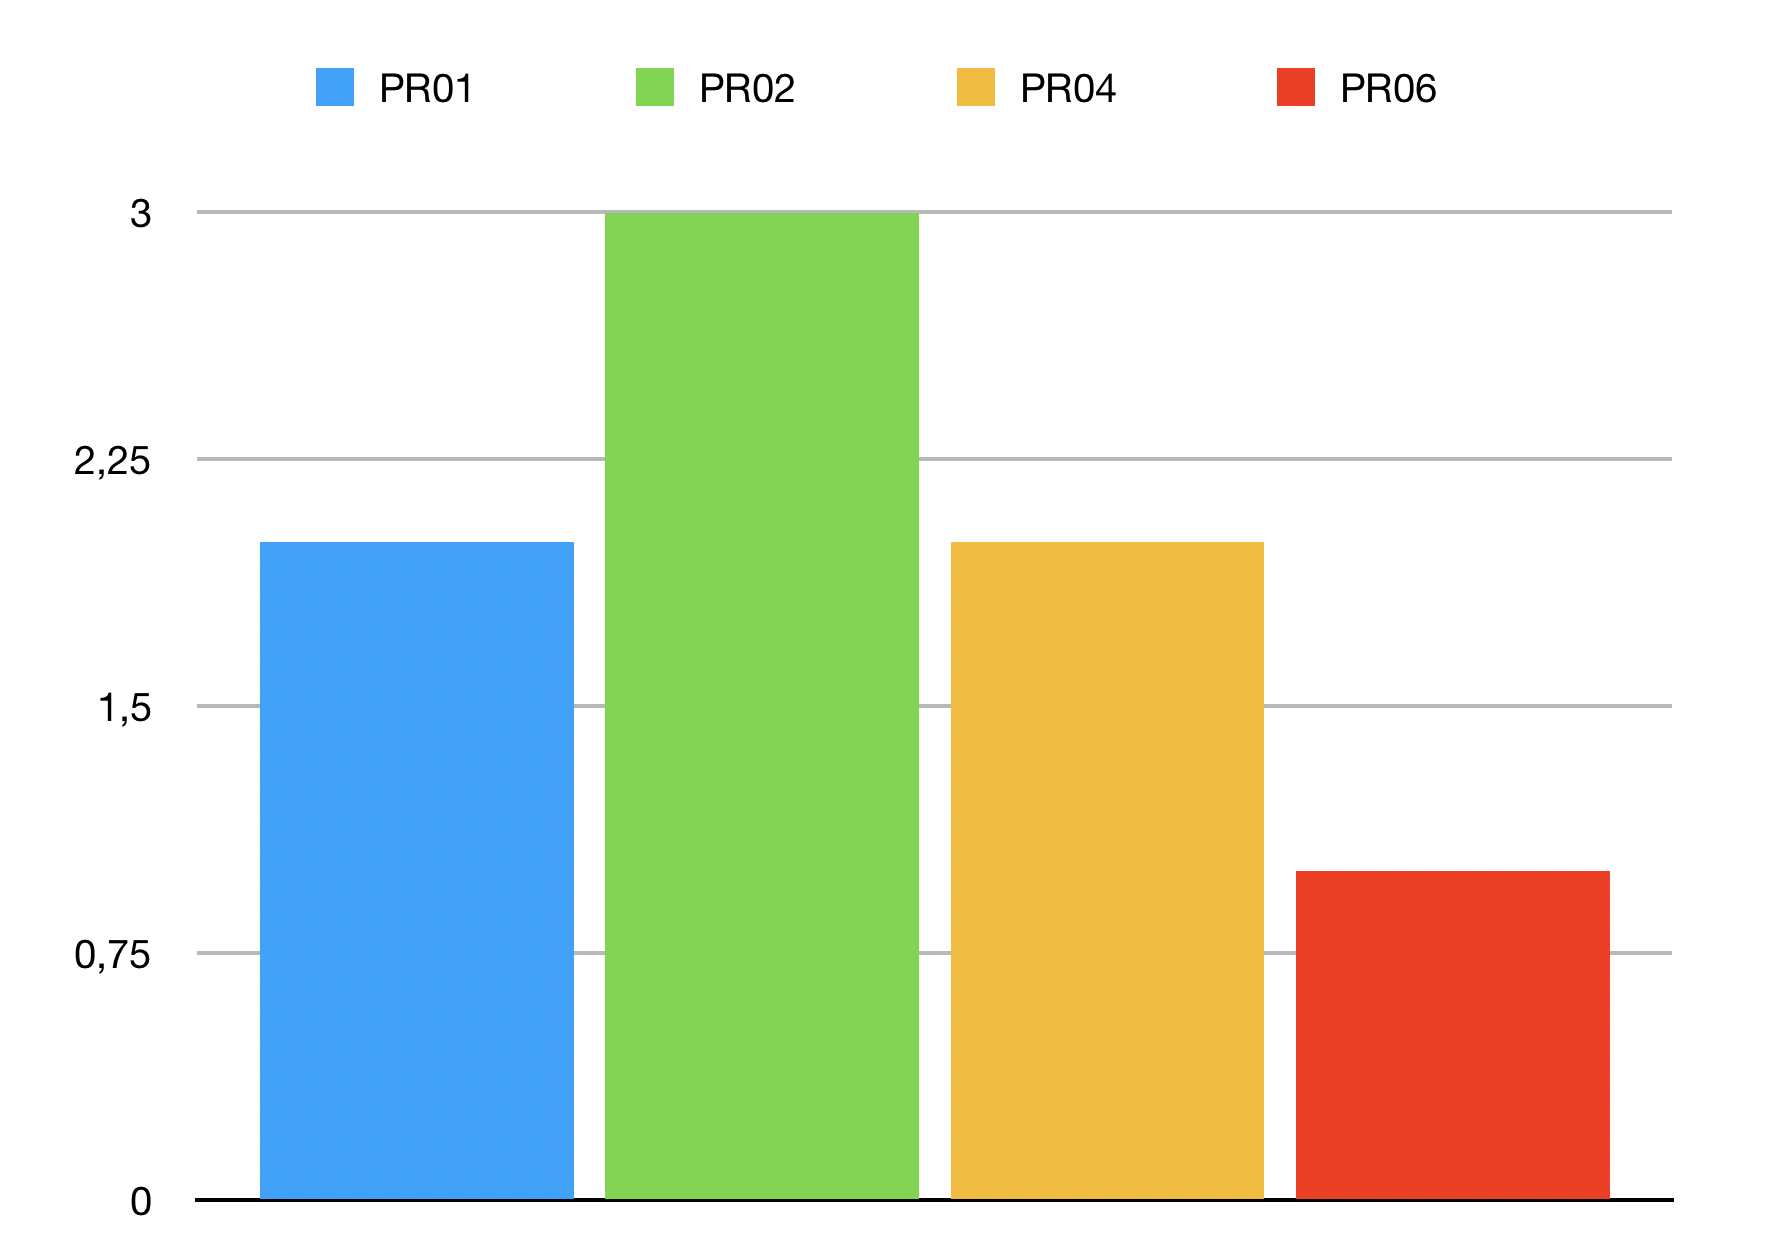
\includegraphics[scale=0.4]{./images/grafici_RP/CMMI.png} 
	\end{center}
	\caption{RP : CMMI}
\end{figure}

\pagebreak

\paragraph{MTPC01: Schedule Variance} ~\\
\begin{figure}[H]
	\begin{center}
		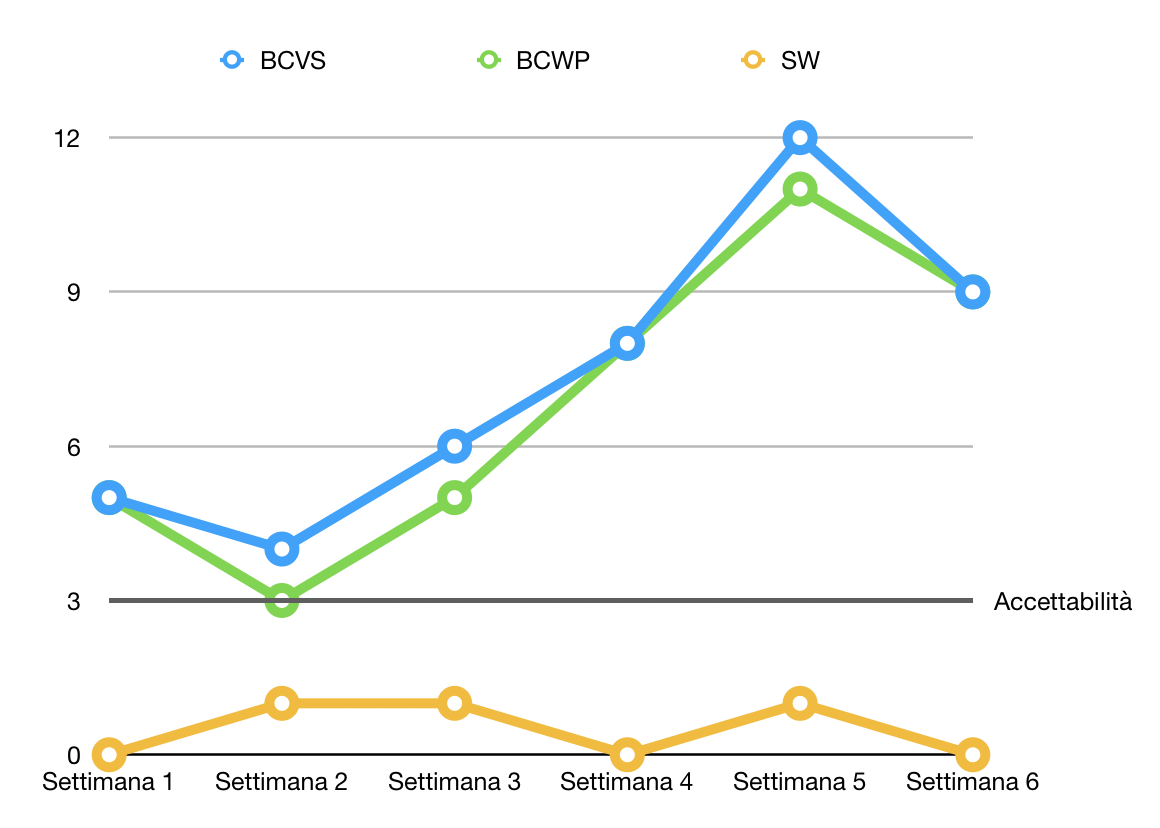
\includegraphics[scale=0.5]{./images/grafici_RP/MTPC01.png} 
	\end{center}
	\caption{RP : MTPC01}
\end{figure}

\paragraph{MTPC02: Budget Variance}\-\\
\begin{figure}[H]
	\begin{center}
		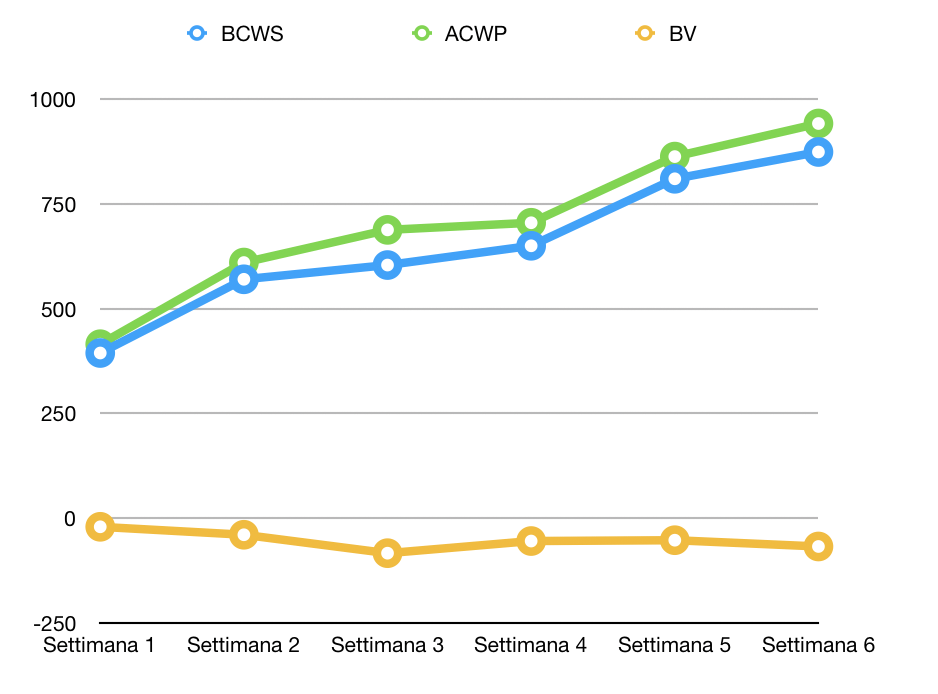
\includegraphics[scale=0.5]{./images/grafici_RP/MTPC02.png} 
	\end{center}
	\caption{RP : MTPC02}
\end{figure}

\pagebreak

\paragraph{MTPC03: Estimated at Completion}\-\\
\begin{figure}[H]
	\begin{center}
		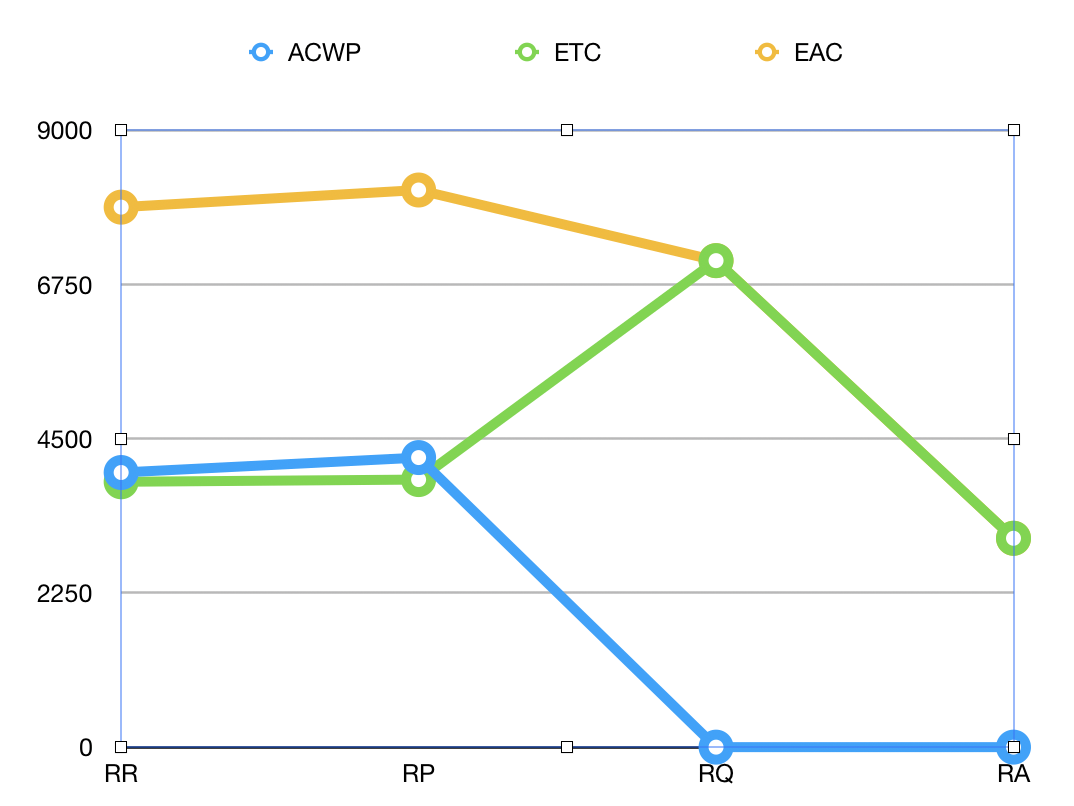
\includegraphics[scale=0.5]{./images/grafici_RP/MTPC03.png} 
	\end{center}
	\caption{RP : MTPC03}
\end{figure}

\paragraph{MTPC14: Media Commit per Settimana}\-\\
\begin{figure}[H]
	\begin{center}
		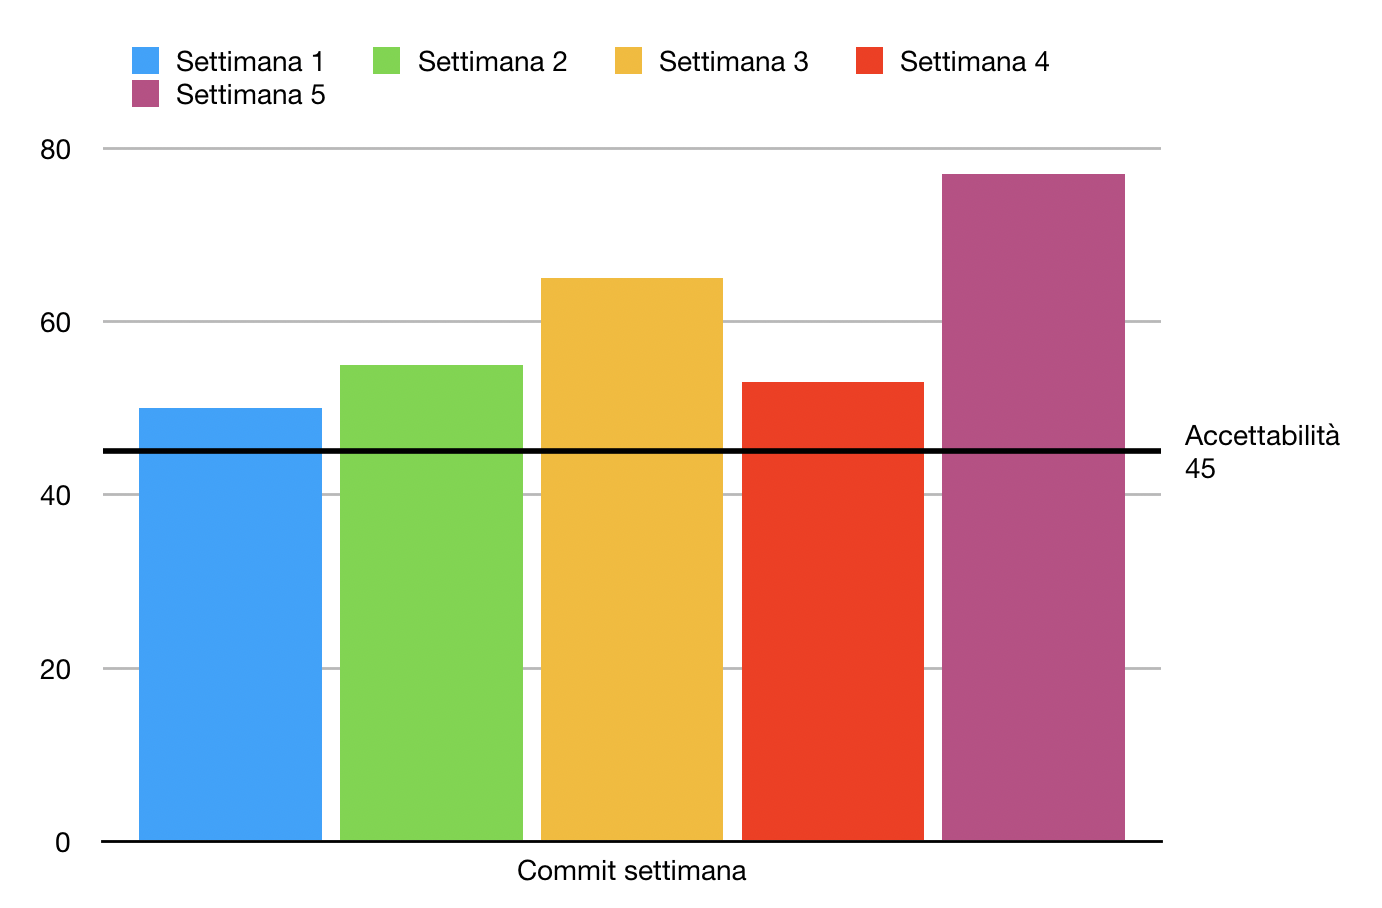
\includegraphics[scale=0.5]{./images/grafici_RP/commitGithub.png} 
	\end{center}
	\caption{RP : MTPC14 - GitHub}
\end{figure}

\begin{figure}[H]
	\begin{center}
		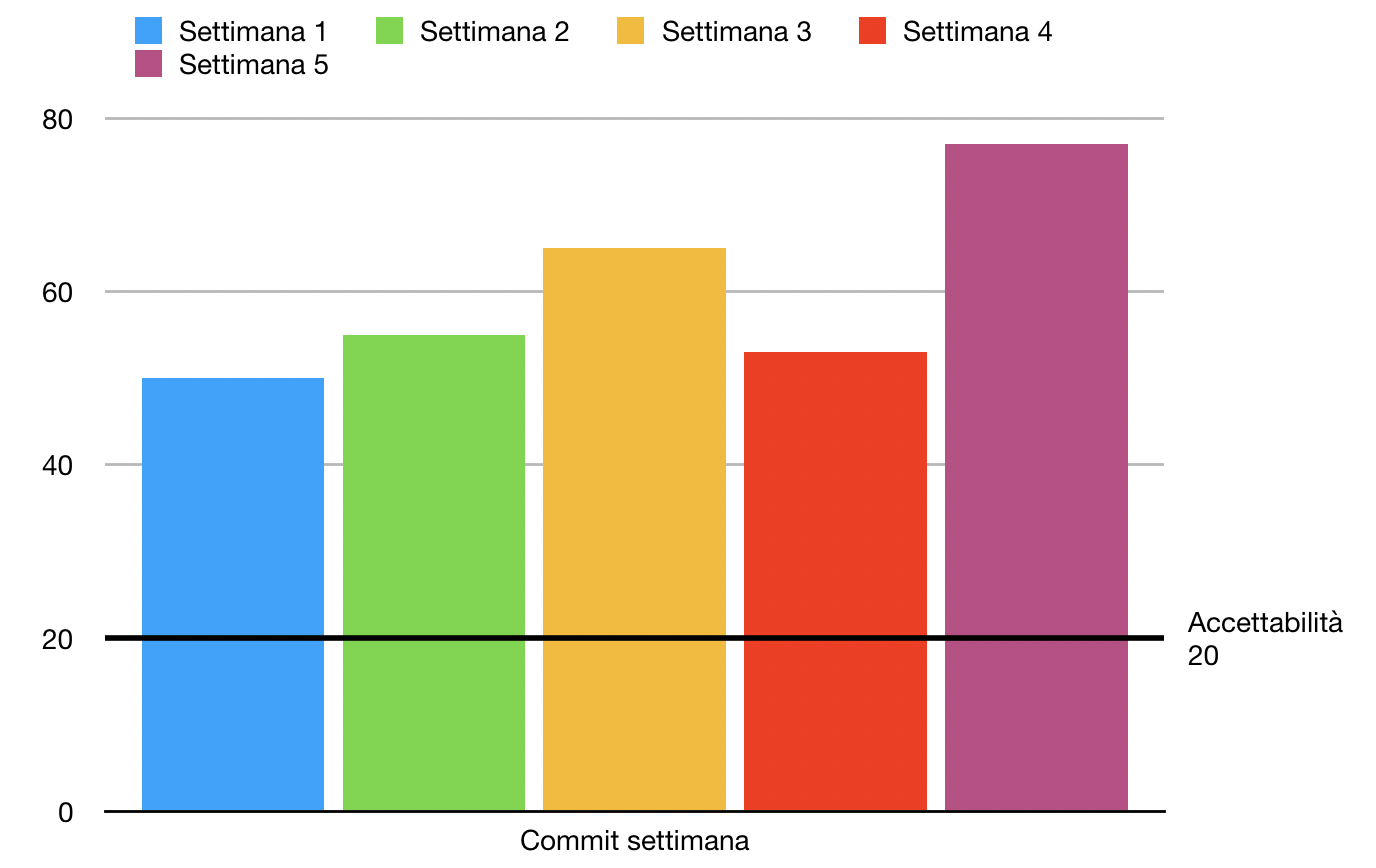
\includegraphics[scale=0.5]{./images/grafici_RP/commitGitlab.png} 
	\end{center}
	\caption{RP : MTPC14 - GitLab}
\end{figure}


\paragraph{MTPC15: Percentuali Build Superate}\-\\
\begin{figure}[H]
	\begin{center}
		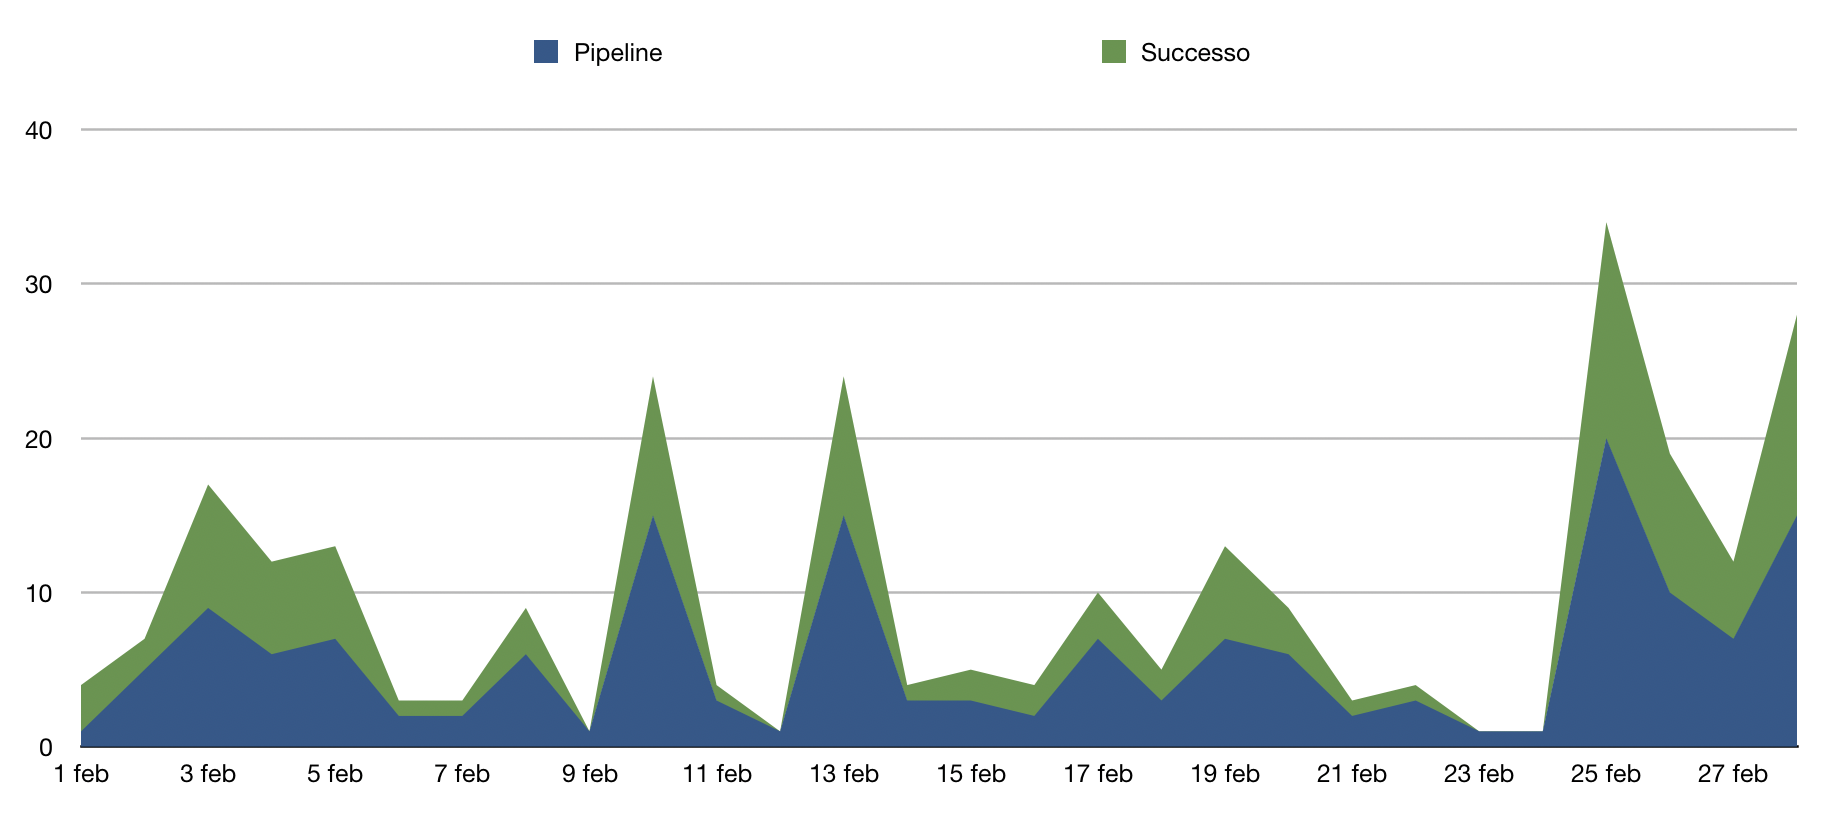
\includegraphics[scale=0.4]{./images/grafici_RP/graficoPipeline.png} 
	\end{center}
	\caption{RP : MTPC15}
\end{figure}

\pagebreak

\paragraph{MTPDD18: Indice di Gulpease}\-\\
\label{gulpi}

\begin{figure}[H]
	\begin{center}
		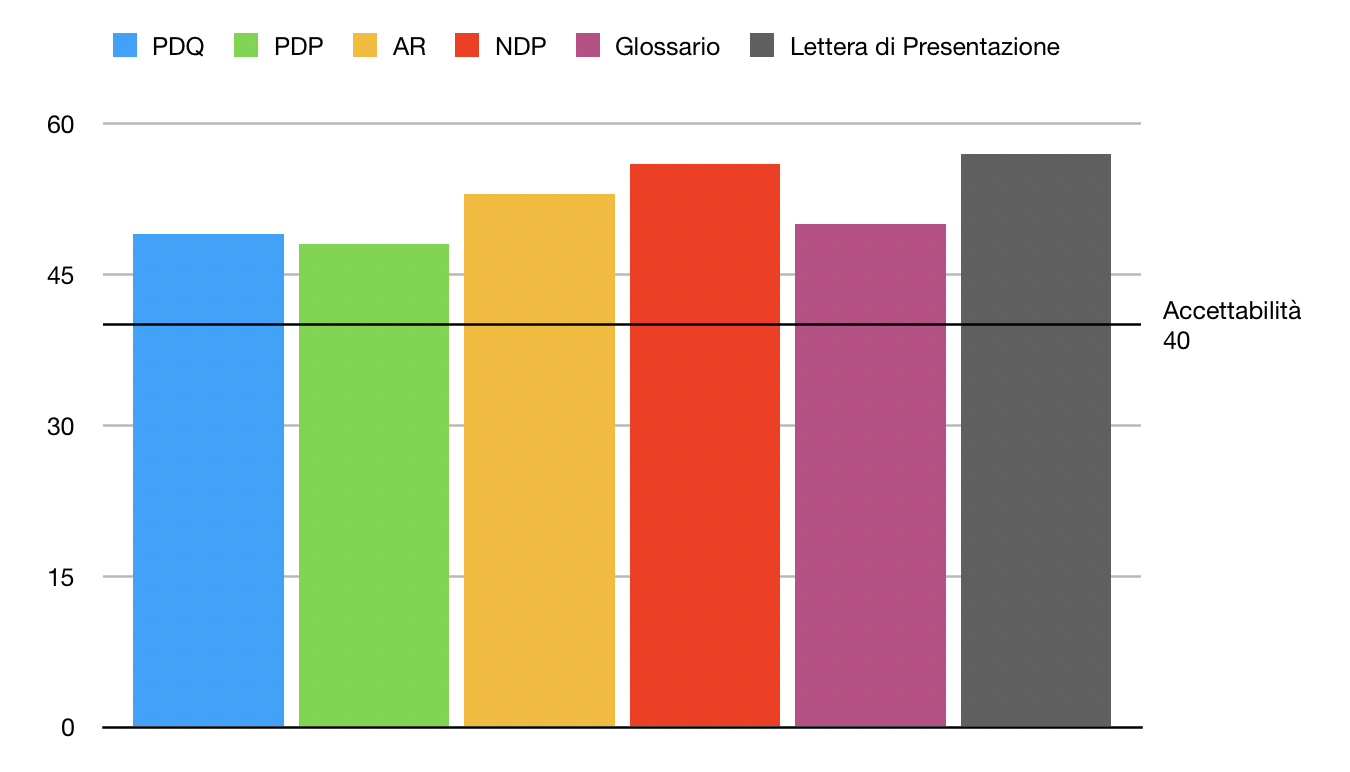
\includegraphics[scale=0.6]{./images/grafici_RP/gulpeasedocumenti.png} 
	\end{center}
	\caption{RP : MTPDD18 - Documentazione}
\end{figure}

\begin{figure}[H]
	\begin{center}
		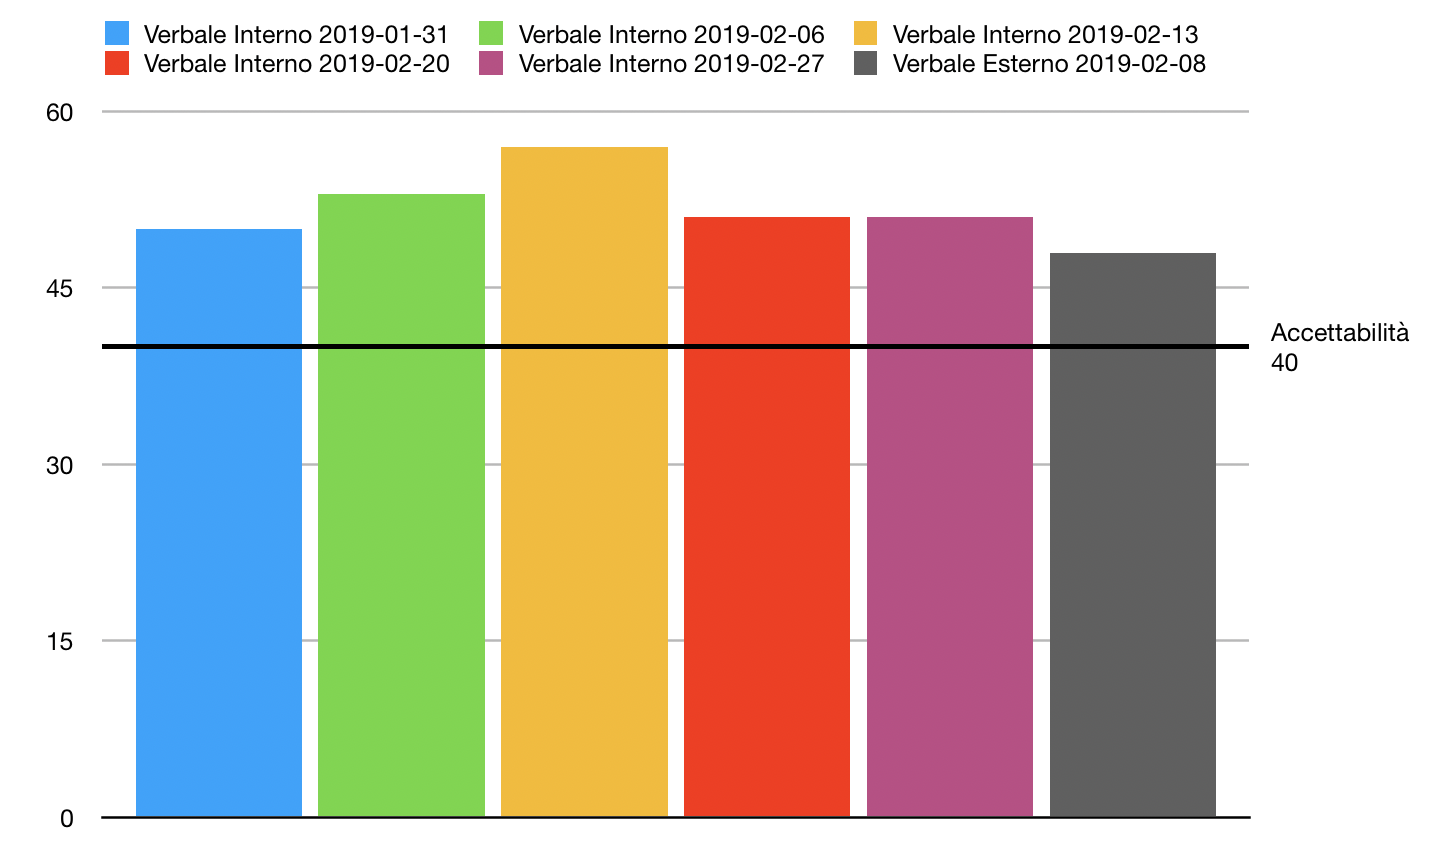
\includegraphics[scale=0.5]{./images/grafici_RP/gulpeaseverbali.png} 
	\end{center}
	\caption{RP : MTPDD18 - Verbali Interni ed Esterni}
\end{figure}


\newpage
\subsection{Revisione di Qualifica}

Questa sezione verrà implementata al termine del periodo di RQ.

\subsection{Revisione di Accettazione}

Questa sezione verrà implementata al termine del periodo di RA.

